% \newpage
\subsection{Планирование отгрузки}
\label{bp:ShipmentPlanning}

При регистрации заявки клиента Менеджер сообщает логисту, что и когда планирует отгружать в форме таблицы Excel (форма \ref{pic:d34}).
Менеджер указывает дату отгрузки в заказе покупателя в системе 1С:УПП.

Каждый день в 10:30 и 14-30 плановик приносит планы работы по ГА и переработке (форма \ref{pic:d12}, \ref{pic:d13}). 
Каждое утро менеджер видит остатки по готовой продукции на складах в системе 1С:УПП.
Менеджер контролирует данные по готовой продукции по складу (форма \ref{pic:d14}).

Менеджер создает заявку на отгрузку в 1С:УПП (форма \ref{pic:d15}) и в проверяет план отгрузки в 1С:УПП (форма \ref{pic:d16}).
Менеджер отправляет распоряжение на отгрузку логисту через 1С:УПП. Логист проверяет складские остатки.

Логист ищет транспорт, указывает параметры машины в 1С:УПП,  формирует сборный груз в транспортных ордерах.
На предприятии есть свой транспорт автомобиль Газель для перевозок по городу.
По городу заявки на перевозку принимаются до 15 часов на следующий день.

На сезон тарифы по перевозке зафиксированы компаниями-перевозчиками. На Владивосток отгрузка производится контейнерами. Отгрузка готовой продукции в Казахстан выполняется только на условиях самовывоза.

Логист относит план отгрузки (форма \ref{pic:d34}) относит на пункт охраны и на склад.
В приоритете отгрузка продукции потребителям по городу Омску.
Логист корректирует план отгрузки (форма \ref{pic:d34}) в соответствии с планом производства.

На предприятии бывает отгрузка готовой продукции в ночное время.

Логист открывает через систему 1С:УПП документ  заказ клиента, проверяет технологическую карту, определяет  габариты транспортного места и рассчитывает вручную план погрузки.

Логист вручную создает схему погрузки готовой продукции в транспорт. 
В системе 1С:УПП не представлена информация по габаритам готовой продукции с поддоном.


\textbf{Сборный груз}

Менеджер  создает заказ на отгрузку в системе 1С:УПП. Логист заполняет в системе 1С:УПП (форма \ref{pic:d34}) в заявку, выбирает водителя и транспорт (форма \ref{pic:d15}).
Если заказ покупателя не уехал полностью, то Менеджер создает в системе 1С:УПП новый заказ клиента.

В форме \ref{pic:d15} на время логист не смотрит.
В системе 1С:УПП программа не  позволяет ставить 3 машины на погрузку на одно время.
Поэтому план отгрузки не совпадает с фактом.

Логист передает на склад формы \ref{pic:d15} и \ref{pic:d34}.


Логист указывает время фактической подачи машины и дату и факт отгрузки в форме \ref{pic:d15}. Таким образом в  1С:УПП видны простои транспорта. 

Логист не использует сервисы для управления транспортом.

Существуют конвейерные отгрузки. 
Заявку на погрузку закрывает в 1C:УПП кладовщик.





% Менеджер пишет задание на отгрузку в чат mail.ru инженерам по отгрузке и формирует заявку (рис. \ref{pic:d22}).

% В СБИС инженер по отгрузке создает план отгрузки (рис. \ref{pic:d22}). 
% Предприятие использует только наемный транспорт или самовывоз транспортом заказчика.
% Менеджер создает план отгрузки  (рис. \ref{pic:d23}) в конце рабочего дня с опозданием на 6 часов и передает в производство мастеру и на склад.
% План отгрузки передается мастеру производства.

% На основании плана отгрузки (рис. \ref{pic:d23}) инженер по отгрузке создает распоряжение на отгрузку в СБИС (рис. \ref{pic:d24}).


% Каждый день до 16:00 (?) МСЗ по плану производства из таблицы MS Excel планирует отгрузку в соответствии с планом производства на основании списка заказов покупателей и остатков ГП (рис. \ref{pic:d17}).
% , \ref{pic:d8}) 
Менеджер факт отгрузки согласовываются с клиентом. %Менеджер планирует отгрузку (рис. \ref{pic:d17}). 


% % Каждый менеджер на основании плана отгрузки (рис. \ref{pic:d17}) пишет заявку на отгрузку (рис. \ref{pic:d10}). 
% Менеджер пишет в чате или сообщает устно логисту о созданном распоряжении.
% Начальник отдела логистики в чате получает пожелания от менеджеров по отгрузке. Почти вся продукция отгружается  на поддонах.
% Начальник отдела логистики получает заявку (рис. \ref{pic:d24}) в системе СБИС.
% На предприятии выделен 1 логист (Начальник отдела логистики). Начальник отдела логистики ищет машины, создает подачи график машин.

% Начальник отдела логистики по заявке на продажу подбирает транспорт.
% % и планирует подачу транспорта на предприятие, разрабатывает график отгрузки. Заявка на отгрузку создается за два дня до отгрузки.
% Начальник отдела логистики составляет план суточный по отгрузке. Время подачи машины не указывается.
% % Для поиска машин для межгорода логисты используют сервис Ati.ru.

% Начальник отдела логистики считает загрузку на фуру по техкарте упаковки (рис. \ref{pic:d26_1}). Начальник отдела логистики создает заявку на транспорт в СБИС (рис. \ref{pic:d27}), вручную заносит в форму плана отгрузки MS Excel (рис. \ref{pic:d25}), передает менеджеру и на склад кладовщикам
% в системе СБИС на основе заявки на транспорт. Начальник отдела логистики указывает водителя и машину в форме \ref{pic:d24}).

% Начальник отдела логистики пишет заявку перевозчику по емайл или по телефону. 
% Факт отгрузки Начальник отдела логистики смотрит по данным системы СБИС, проверяет факт отгрузки готовой продукции.
 

% Инженер по отгрузке в системе СБИС формирует пропуск (распоряжение на отгрузку), указывает машину из формы \ref{pic:d25} в СБИС.





% \begin{figure}
% \begin{center}
%   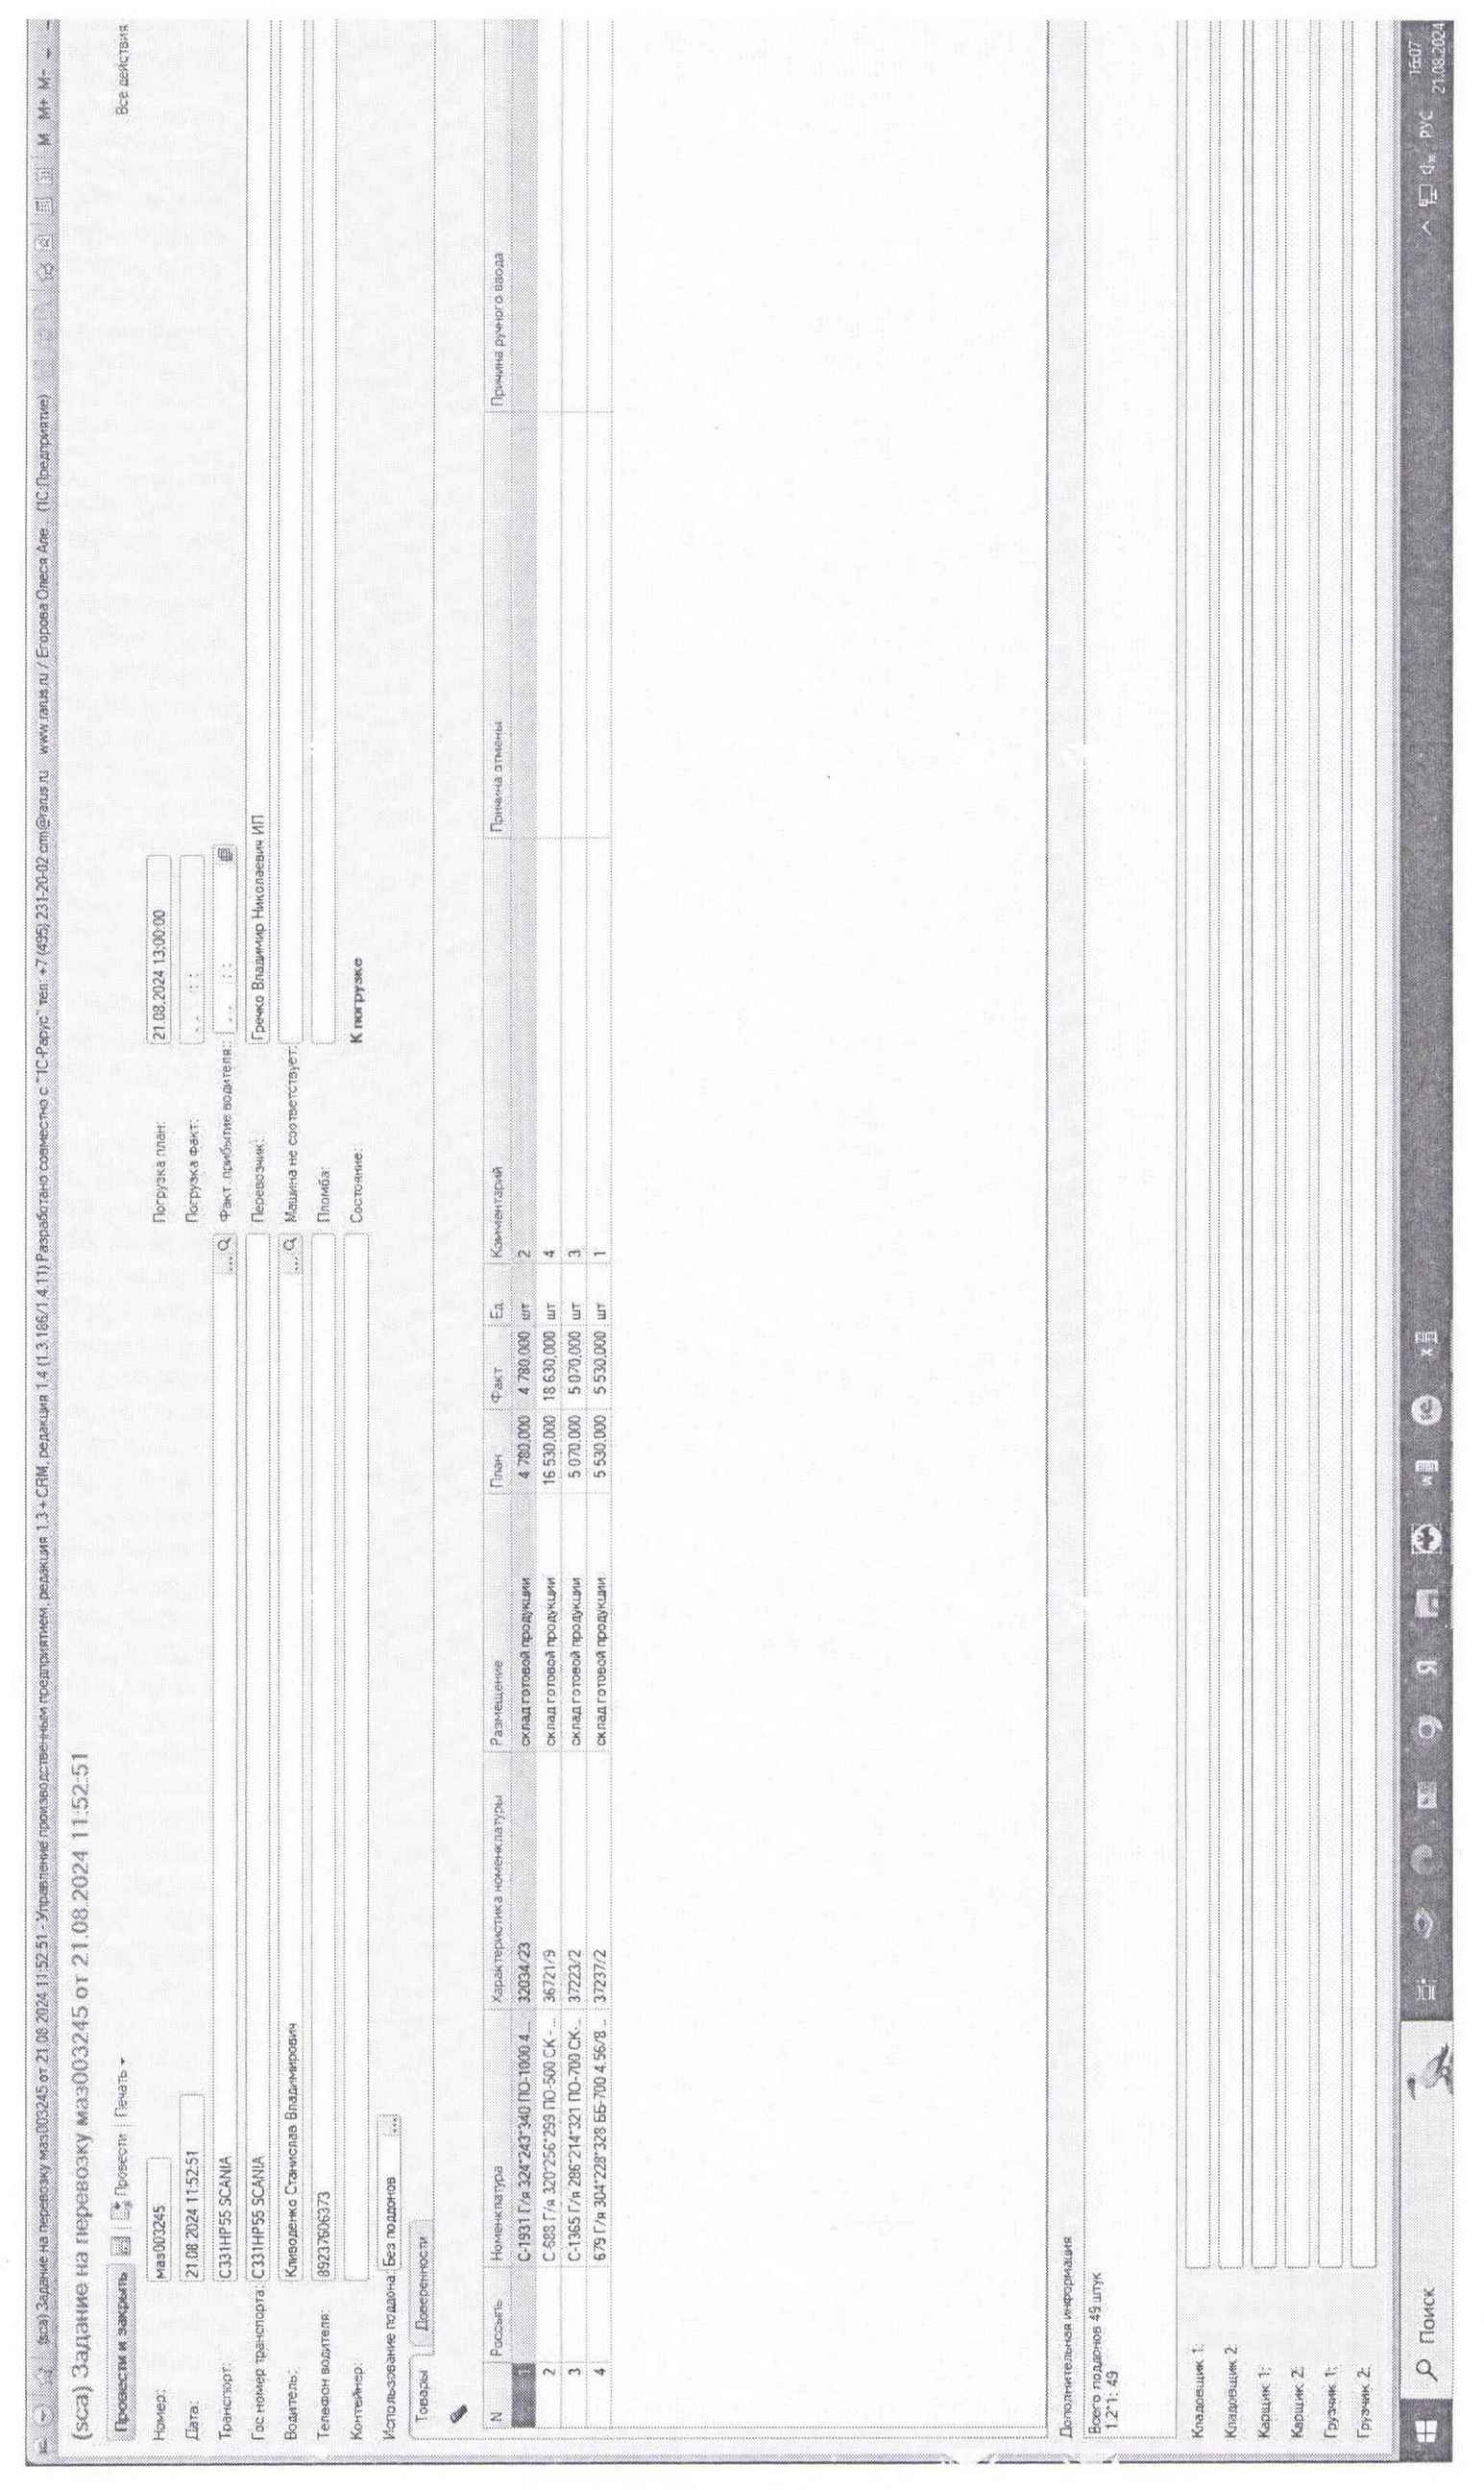
\includegraphics[height=0.8\textheight, width=\textwidth, keepaspectratio]{Pics/d25.jpg}
% \end{center}
%   \caption{План отгрузки готовой продукции}
%   \label{pic:d25}
% \end{figure}

% \begin{figure}
% \begin{center}
%   \includegraphics[height=0.94\textheight, width=\textwidth, keepaspectratio]{Pics/d26_1.jpg}
% \end{center}
%   \caption{Технологическая карта на отгрузку}
%   \label{pic:d26_1}
% \end{figure}

% \begin{figure}
% \begin{center}
%   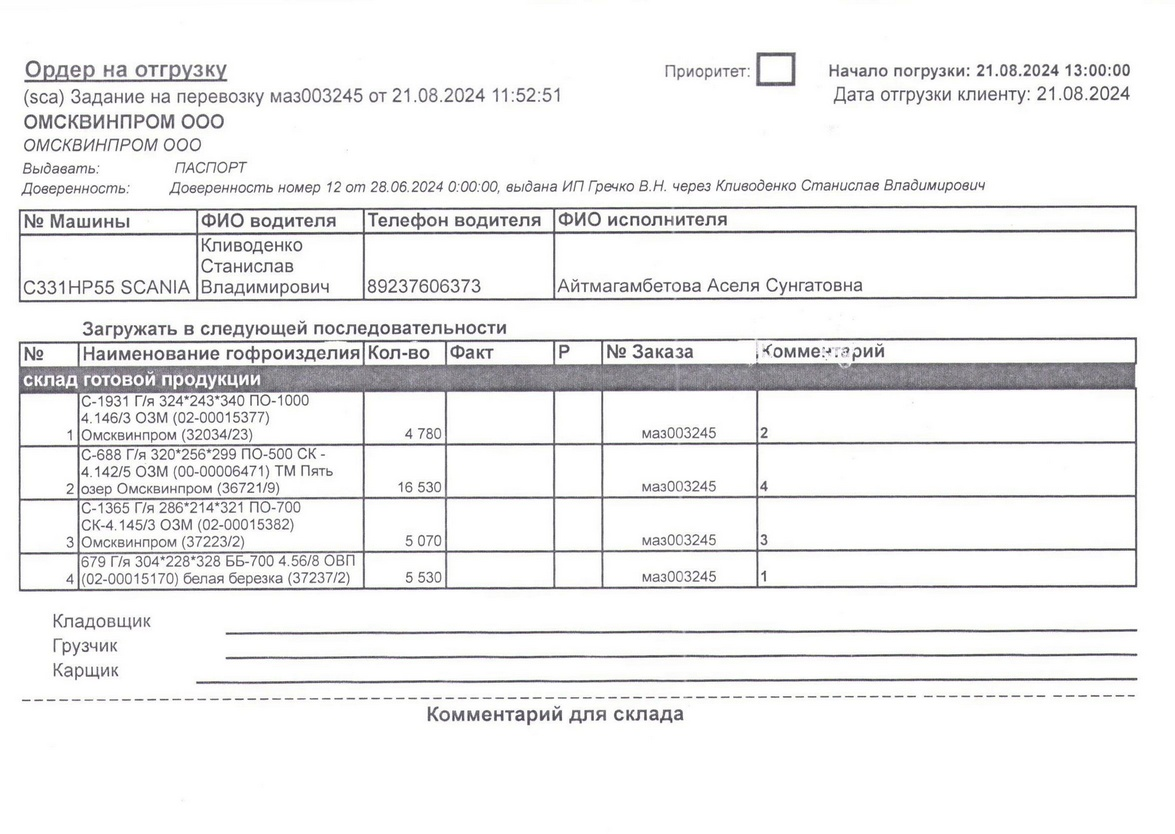
\includegraphics[height=0.94\textheight, width=\textwidth, keepaspectratio]{Pics/d27.jpg}
% \end{center}
%   \caption{Форма заявки на транспорт в СБИС}
%   \label{pic:d27}
% \end{figure}


%Менеджеры отдела продаж контролируют выпуск готовой продукции по появлению остатков ГП. Контроль остатков ведется в файле MS Excel \ref{pic:11_stockGPexcel}. 
%Остатки по ГП актуальны на следующий день после производства к 10:00. 
%Поскольку на предприятии выделены два юридических лица, то менеджеры контролируют остатки по ГП по обеим юридическим лицам. 
%
%Менеджеры отдела продаж ведут файл плана отгрузки \ref{pic:10_shipping_plan1} в электронном виде в формате Excel.
%План отгрузки менеджер формирует на основании заявок на производство \ref{pic:09_OrederToProduction}, где указана желаемая и согласованная дата отгрузки.
%
%План отгрузки в электронном виде находится в сетевом доступе.
%Согласованный план отгрузки менеджер передает логисту для планирования транспорта.
%
%Логист постоянно контролирует файл плана отгрузки \ref{pic:10_shipping_plan1}, определяет на основании плана отгрузки транспорт и формирует план отгрузки с учетом поставки транспорта \ref{pic:10_shipping_plan2}. 
%Логист корректирует планы отгрузки \ref{pic:10_shipping_plan2}, указывает транспортное средство и время прибытия, адреса доставки.
%На предприятии существует собственный транспорт. В сутки собственный транспорт делает от 4 до 10 поездок.
%Согласованный логистом план отгрузки передается на склад в электронном виде через сетевой каталог.
%
%На основании плана отгрузки \ref{pic:10_shipping_plan2} логист формирует заявки сторонним экспедиторам на поставку транспорта \ref{pic:12_application_for_forwarder}, которые отправляются по электронной почте. Логист должен заказать автотранспорт за один-два дня до отгрузки.
%
%Выделены отгрузка авто и жд транспортом (контейнеры). В месяц формируется до 8 контейнеров с ГП. При контейнерной отгрузке  логист должен заказывать у логистической компании контейнер за 10 дней до отгрузки. 
%
%
%
%Менеджер контролирует отгрузку в программе 1С по отчету по продажам либо по журналу реализации. Менеджер корректирует планы отгрузки по факту отгрузки.
%
%
\begin{figure}
\begin{center}
 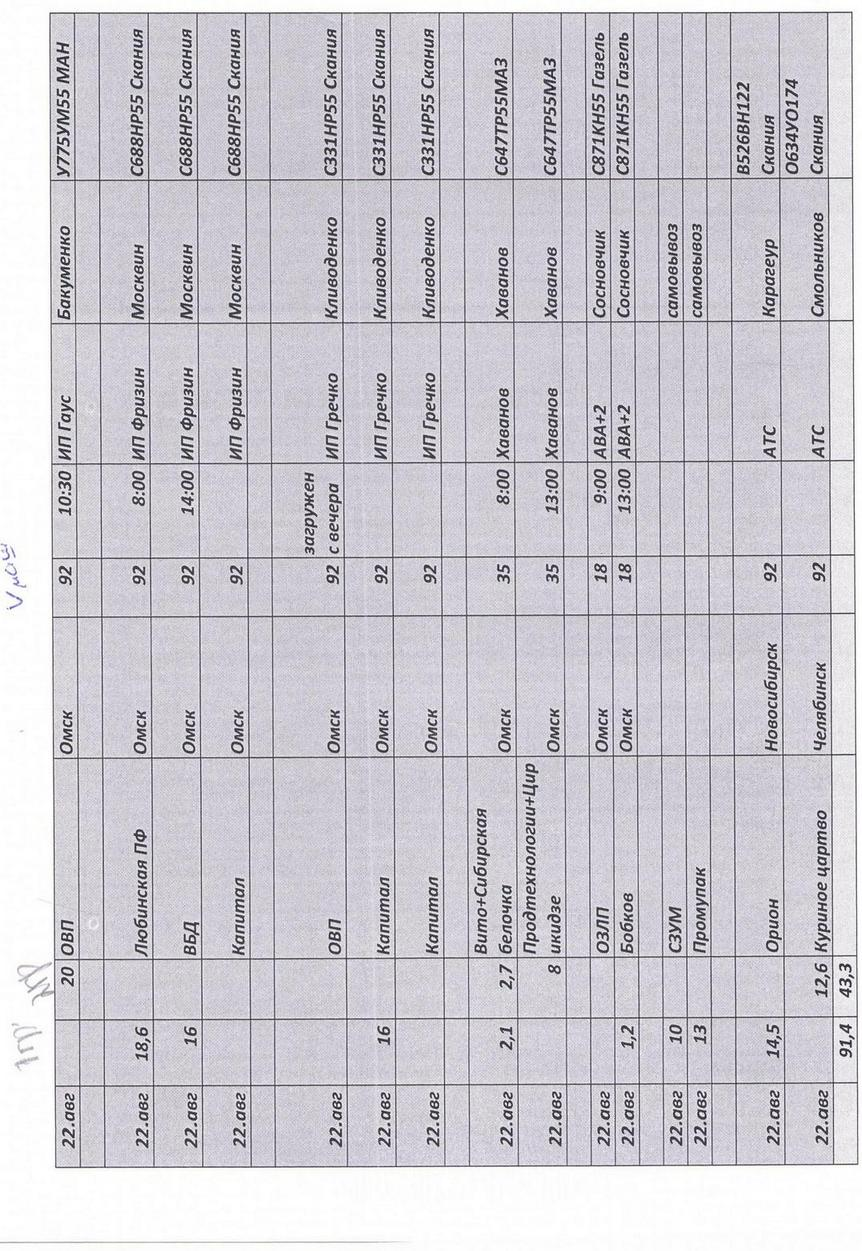
\includegraphics[width=\linewidth, height=0.94\textheight, keepaspectratio]{Pics/d34.jpg}
\end{center}
 \caption{План отгрузки}
 \label{pic:d34}
\end{figure}

\begin{figure}
\begin{center}
 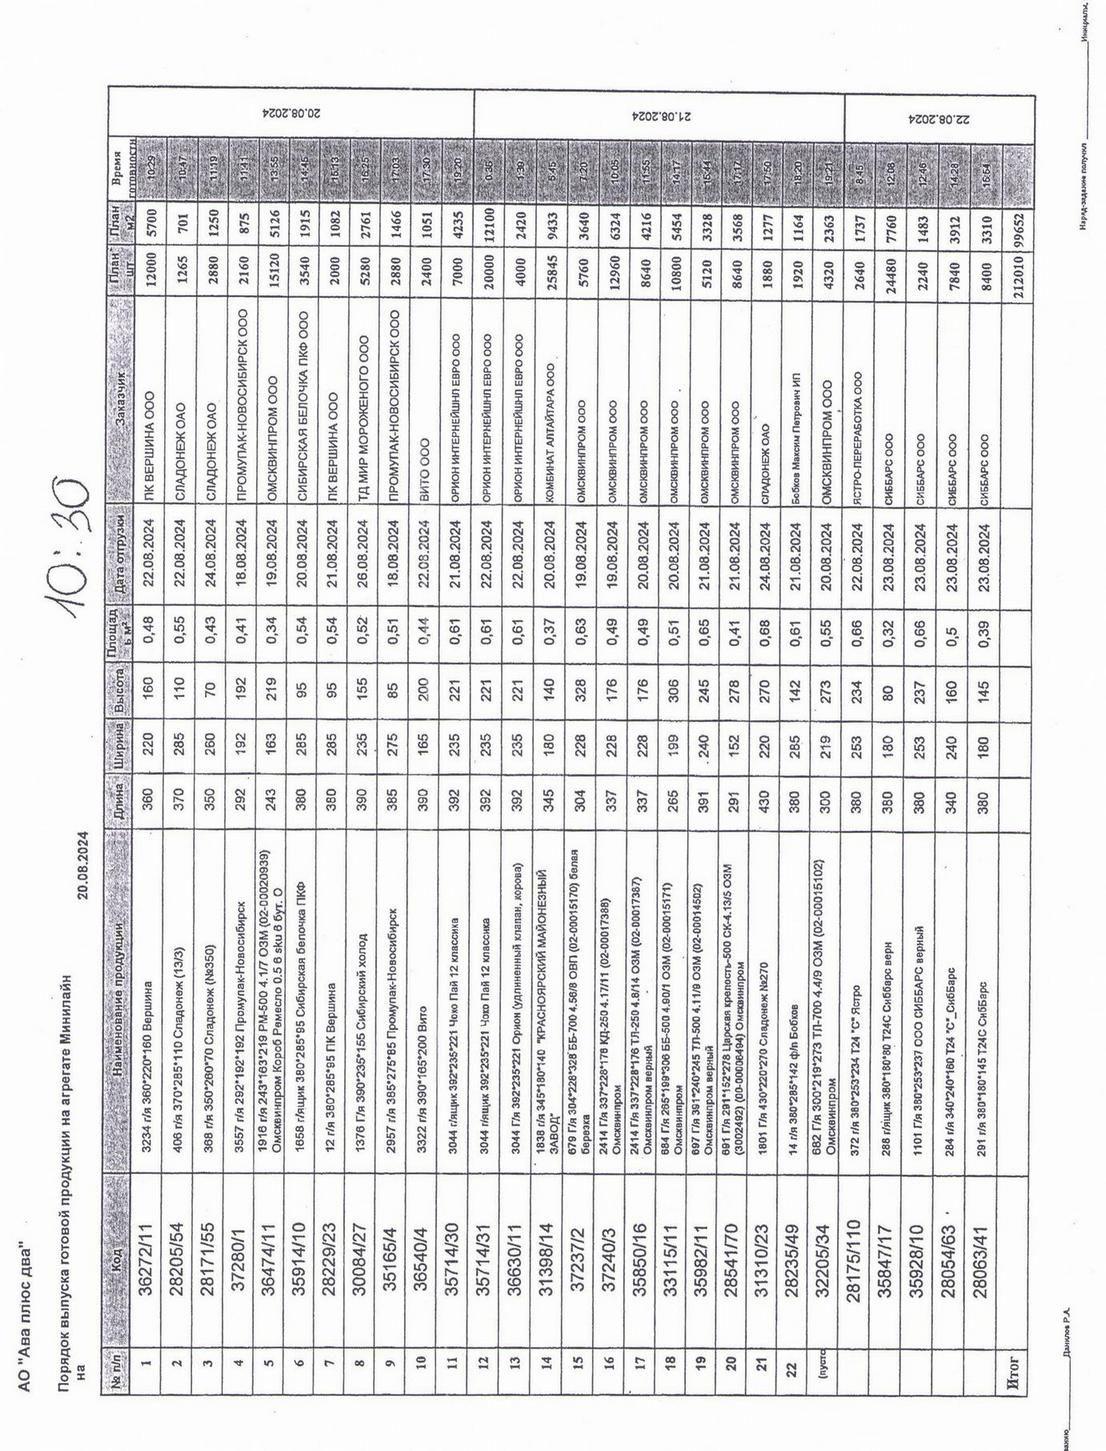
\includegraphics[width=\linewidth, height=0.94\textheight, keepaspectratio]{Pics/d12_2.jpg}
\end{center}
 \caption{Задание на гофроагрегат, экземпляр для менеджеров}
 \label{pic:d12}
\end{figure}

\begin{figure}
\begin{center}
 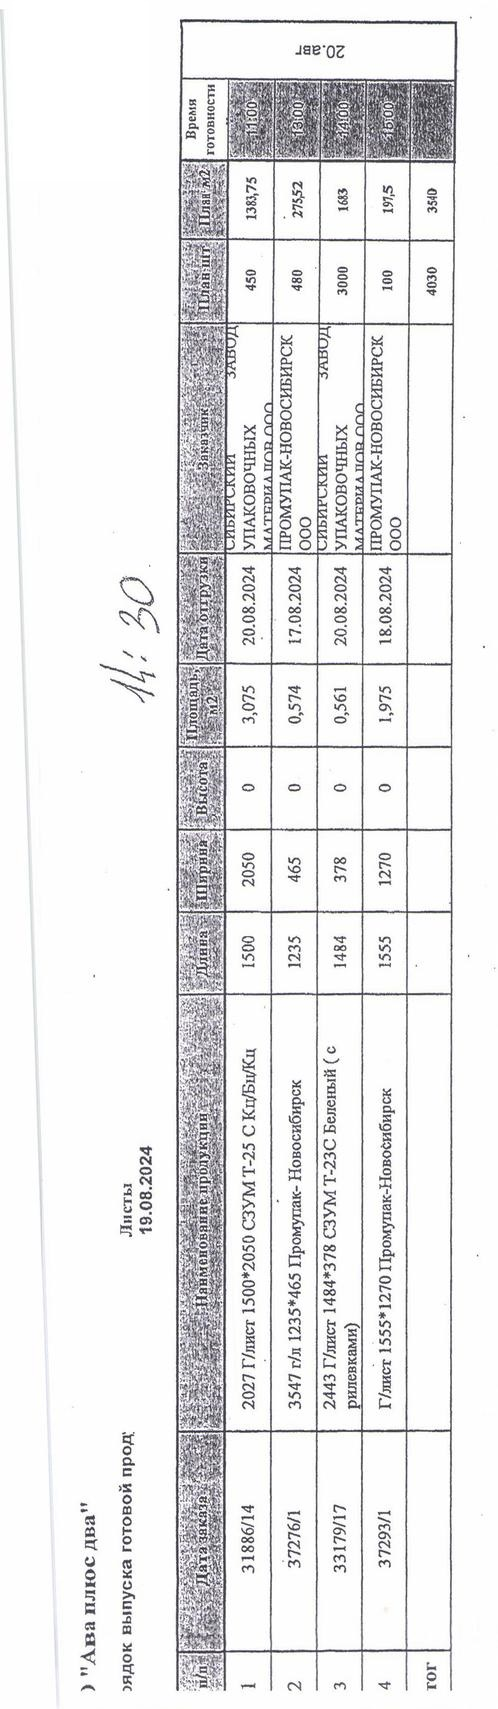
\includegraphics[width=\linewidth, height=0.94\textheight, keepaspectratio]{Pics/d13.jpg}
\end{center}
 \caption{Задание на линии переработки, экземпляр для менеджеров}
 \label{pic:d13}
\end{figure}


\begin{figure}
\begin{center}
 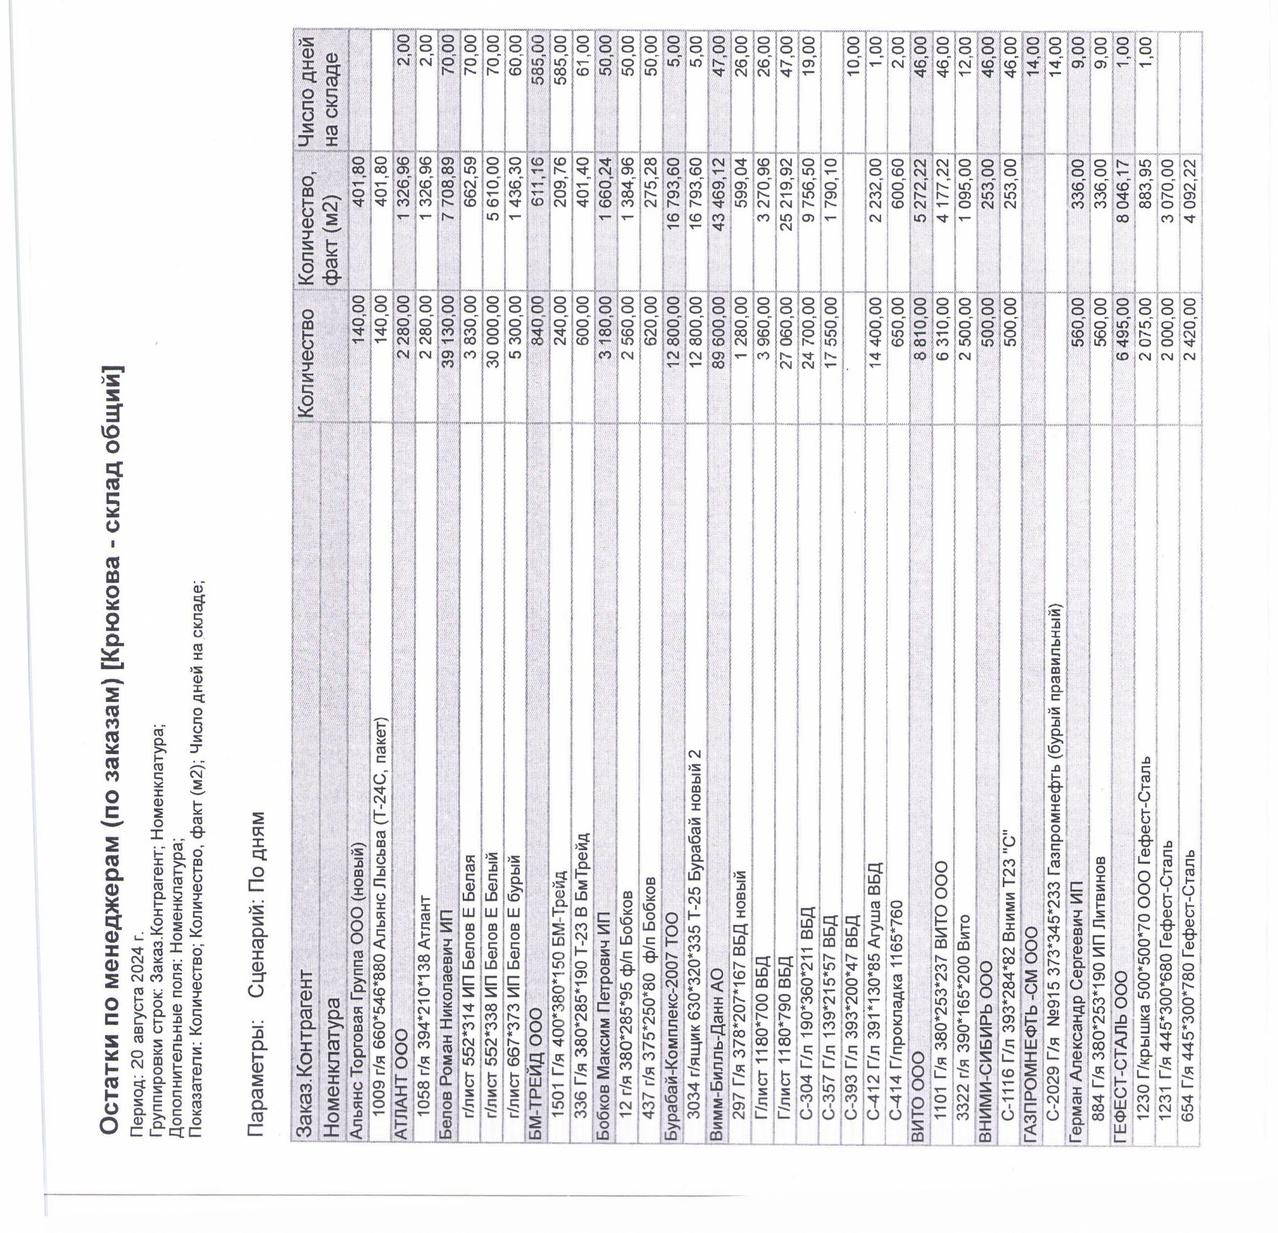
\includegraphics[width=\linewidth, height=0.94\textheight, keepaspectratio]{Pics/d14.jpg}
\end{center}
 \caption{Форма остатков готовой продукции для менеджеров}
 \label{pic:d14}
\end{figure}

\begin{figure}
\begin{center}
 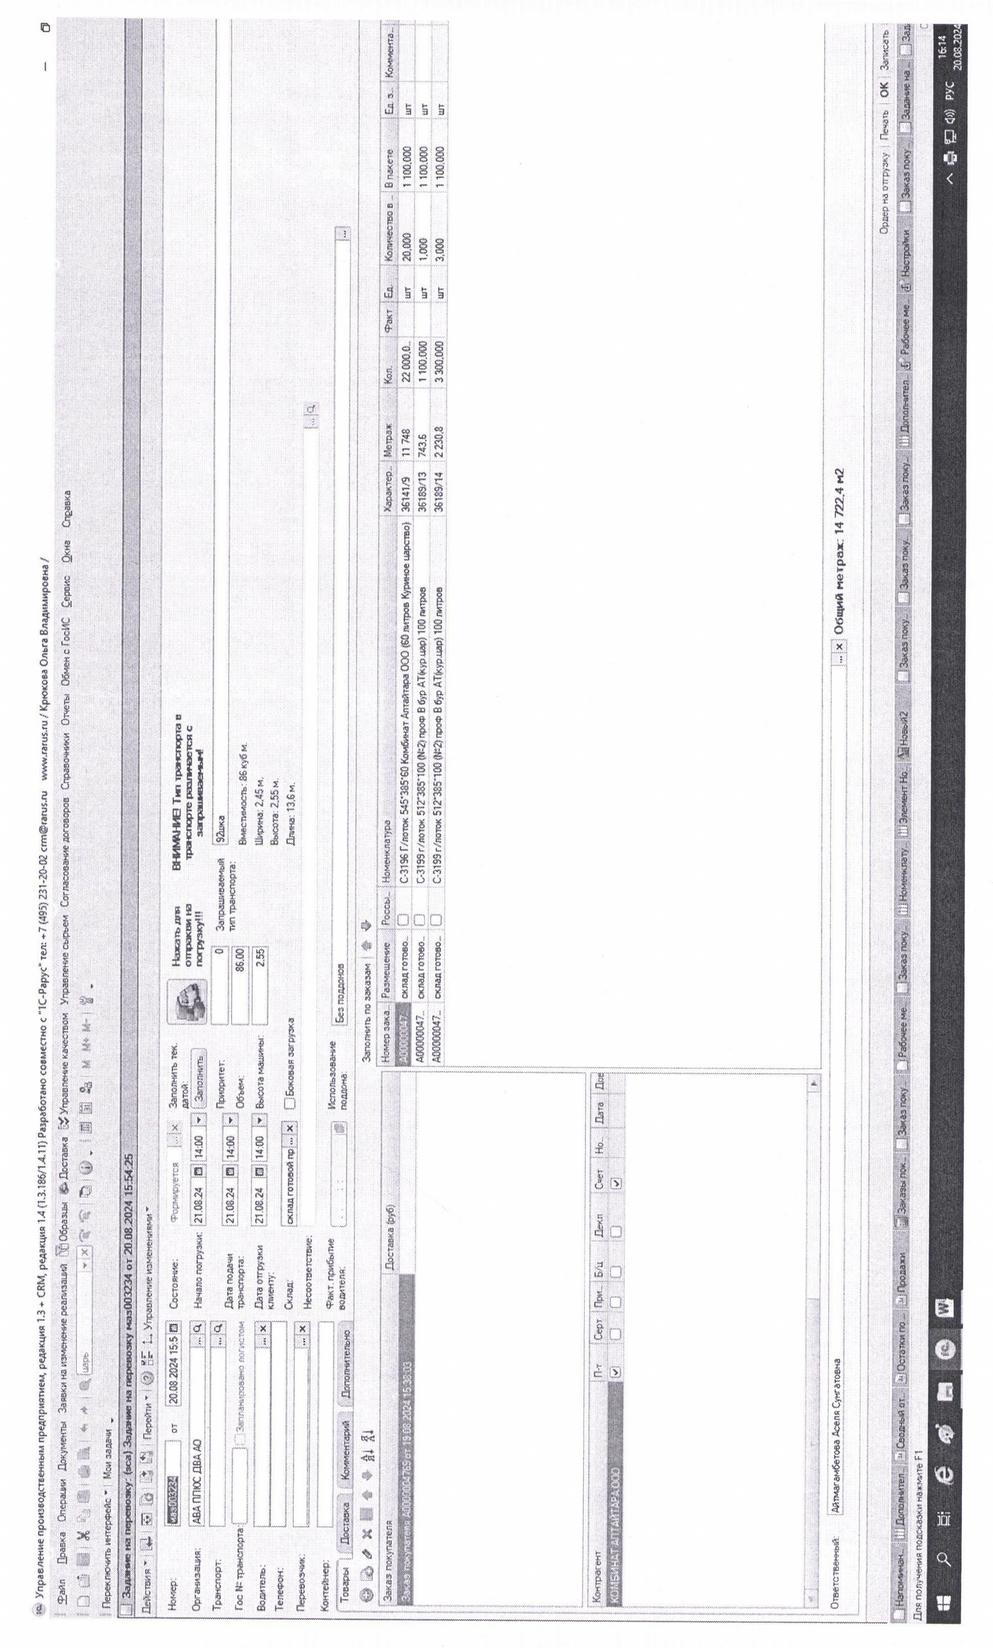
\includegraphics[width=\linewidth, height=0.94\textheight, keepaspectratio]{Pics/d15.jpg}
\end{center}
 \caption{Форма заявки на отгрузку в 1С:УПП}
 \label{pic:d15}
\end{figure}

\begin{figure}
\begin{center}
 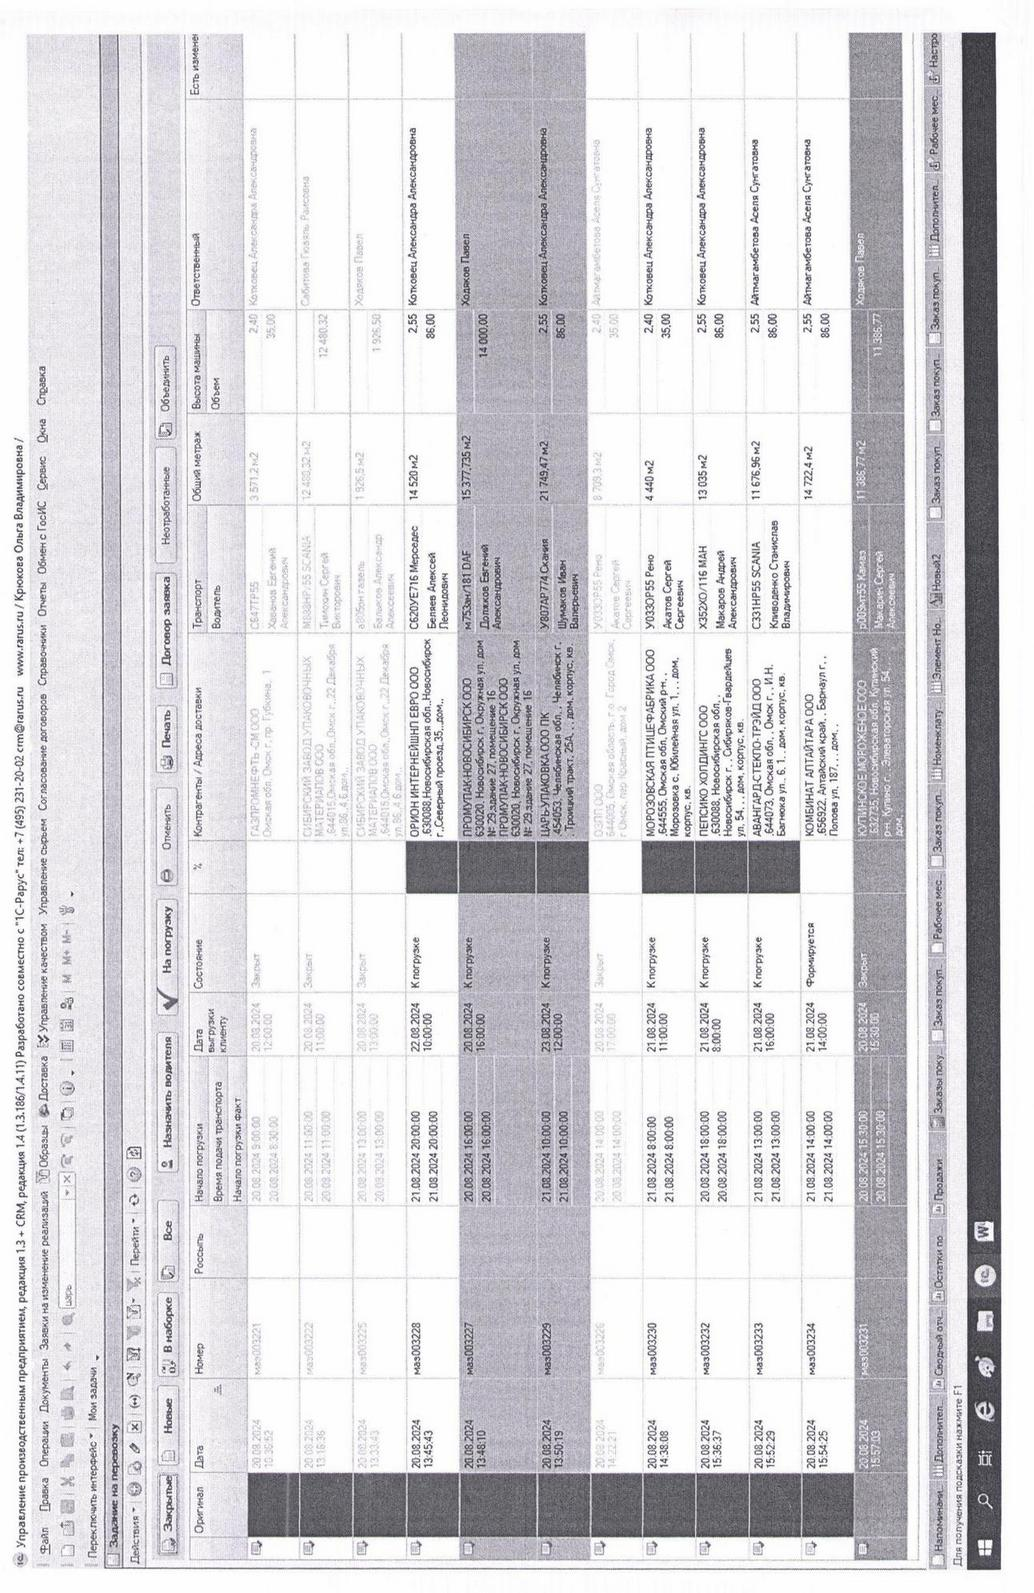
\includegraphics[width=\linewidth, height=0.94\textheight, keepaspectratio]{Pics/d16.jpg}
\end{center}
 \caption{Форма плана отгрузки в 1С:УПП}
 \label{pic:d16}
\end{figure}